\documentclass[10pt,a4paper]{article}
\usepackage[margin=2cm]{geometry}
\usepackage[T1]{fontenc}
\usepackage{lmodern}
\usepackage{microtype}
\usepackage{graphicx}
\usepackage{booktabs}
\usepackage{tabularx}
\usepackage{xcolor}
\usepackage{amsmath}
\usepackage{caption}
\usepackage{enumitem}
\usepackage[hidelinks]{hyperref}
\setlist{nosep,leftmargin=*}
\captionsetup{font=small}
\newcommand{\pending}[1]{\textcolor{red}{[PENDING: #1]}}
\sloppy\emergencystretch=3em
\renewcommand{\path}[1]{\texttt{#1}}

\title{Instruction Tuning and DPO on Qwen2.5-0.5B}
\author{Usman Naeem (25280021)}
\date{PA2, Advanced GenAI \& Agents}

\begin{document}
\maketitle
\vspace{-1.5em}

\section{Repository, Models, and Data}

\textbf{Repository.} \url{https://github.com/usmanbinnaeem/small-model-alignment-starter}. The core code
(batching, log-probabilities, SFT and DPO loss) is in \texttt{smalign/}, and the training, generation and judging scripts
are in \texttt{scripts/}. \texttt{submission\_adapter.py} only calls into \texttt{smalign}. The 7 public tests pass, and
I added 17 more tests in \texttt{tests/} for truncation, padding, row order and resuming. The Kaggle notebooks are made
by \texttt{kaggle/build\_notebooks.py}.

\textbf{Models.} Base checkpoint \texttt{Qwen/Qwen2.5-0.5B}. Persona task: \texttt{HuggingFaceTB/SmolLM2-360M-Instruct}.

\textbf{Data.} \texttt{scripts/prepare\_data.py} builds every subset with seed 42, and the counts are saved in
\texttt{data/prepared\_manifest.json}. I kept only single-turn examples. After filtering, the rows are shuffled with
\texttt{random.Random(42)}, so the same seed always gives the same subset.

\begin{center}\small
\setlength{\tabcolsep}{4pt}
\begin{tabularx}{\linewidth}{l>{\raggedright\arraybackslash}X>{\raggedright\arraybackslash}Xrrr}
\toprule
Track & Source (train / validation split) & Filters & Pool & Train & Val \\
\midrule
SFT & \texttt{ultrachat\_200k} (train\_sft / test\_sft) & first turn; prompt $\le$ 256 tokens; prompt, response and EOS fit in 512 & 104,795 & 30,000 & 1,000 \\
HH DPO & \texttt{Anthropic/hh-rlhf} (train / test) & one Human and one Assistant turn; identical prompts; chosen $\ne$ rejected & 49,029 & 15,000 & 1,000 \\
UF DPO & \texttt{ultrafeedback\_binarized} (train\_prefs / test\_prefs) & score chosen $>$ rejected; prompt $\le$ 256 tokens & 42,861 & 15,000 & 1,000 \\
Persona & \texttt{ramsay\_style\_preferences.json} & seeded split & 220 & 200 & 20 \\
\bottomrule
\end{tabularx}
\end{center}

\textbf{Evaluation sets.} For HH DPO I used the provided \texttt{eval\_sets/hh\_rlhf\_eval\_300\_seed42.json} (300
prompts in 10 categories). For UF DPO I made \texttt{eval\_sets/alpaca\_eval\_300\_seed42.json} by taking
\texttt{sorted(random.Random(42).sample(range(805), 300))} from \texttt{tatsu-lab/alpaca\_eval}. No persona set was given,
so I wrote \texttt{eval\_sets/persona\_style\_eval\_40.json}: 10 prompts each for cooking, coding, general help and
safety-sensitive requests. None of them are in the training data.

\textbf{Prompt format.} I used the same ChatML prompt for SFT, DPO and generation:
\begin{center}\footnotesize\ttfamily
<|im\_start|>system\textbackslash nYou are a helpful assistant.<|im\_end|>\textbackslash n<|im\_start|>user\textbackslash n\{instruction\}<|im\_end|>\textbackslash n<|im\_start|>assistant\textbackslash n
\end{center}
After it comes the response and then the EOS token (\texttt{<|endoftext|>}). I tokenize the prompt and the response
separately and join them, so I know exactly where the response starts. Prompt and padding positions get label $-100$.
Padding is masked by position and not by token id, because in Qwen the PAD token is the same as EOS, and masking by id
would also remove the real EOS label. For the persona task I used SmolLM2's own chat template, because TRL uses it in
training.

\section{Experimental Configuration}

\begin{center}\small
\setlength{\tabcolsep}{4pt}
\begin{tabularx}{\linewidth}{l>{\raggedright\arraybackslash}X>{\raggedright\arraybackslash}X>{\raggedright\arraybackslash}X>{\raggedright\arraybackslash}X}
\toprule
 & SFT & HH DPO & UF DPO & Persona LoRA-DPO (v6) \\
\midrule
Trainable params & full (494M) & full & full & LoRA r 16, $\alpha$ 32, dropout 0.05, q/k/v/o/gate/up/down (8.7M) \\
Loop & own PyTorch loop & own PyTorch loop & own PyTorch loop & TRL 1.15 \texttt{DPOTrainer}, PEFT 0.21 \\
Optimizer & AdamW (0.9, 0.999) & AdamW & AdamW & AdamW (TRL default) \\
Peak LR, schedule & 2e-5, 3\% warmup, cosine & 1e-6 fixed & 1e-6 fixed & 1e-4, 10\% warmup, cosine \\
Weight decay, clip & 0.1 (matrices only), 1.0 & 0, 1.0 & 0, 1.0 & 0, 1.0 \\
Batch & 2 $\times$ 16 accum = 32 & 1 $\times$ 32 = 32 & 1 $\times$ 32 = 32 & 4 $\times$ 2 = 8 \\
Precision & fp16 autocast, fp32 weights, GradScaler & same; reference fp32 on cuda:1 & same & fp16 \\
Max length / prompt & 512 / 256 & 512 / 256 & 512 / 256 & 256 \\
Steps (epochs) & 938 (1) & 469 (1) & 469 (1) & 75 (3) \\
$\beta$, loss & response NLL & 0.1, sigmoid & 0.1, sigmoid & 0.5, sigmoid + SFT (weights 1, 1) \\
Reference & n/a & SFT best (step 938) & SFT best (step 938) & base model, adapter disabled \\
Checkpoint selection & lowest val loss & best val reward acc & best val reward acc & final \\
Seed & 42 & 42 & 42 & 42 \\
\bottomrule
\end{tabularx}
\end{center}

\textbf{SFT loss reduction.} I used the mean negative log-likelihood over all response tokens in a micro-batch, and
the 16 micro-batch losses are averaged for each optimizer step. For DPO, if two checkpoints have the same validation
reward accuracy, the one with the higher margin is kept.

\textbf{Generation.} Greedy decoding with \texttt{max\_new\_tokens} 512 and \texttt{repetition\_penalty} 1.1, no
n-gram blocking, stopping at \texttt{<|endoftext|>} or \texttt{<|im\_end|>}. SFT and DPO always use exactly the same
settings. The persona comparison uses plain greedy decoding with 256 new tokens, the same for every variant and for the
base model.

\section{Parameter Choices and Deviations}

\begin{center}\small
\begin{tabularx}{\linewidth}{llXl}
\toprule
Setting & Guide $\rightarrow$ ours & Reason and evidence & Kind \\
\midrule
SFT data filter & not given $\rightarrow$ must fit in 512 with EOS & So every target ends with EOS and the model learns to stop. This keeps about half of the first turns and makes the SFT data shorter on average. & data \\
UF ties & not given $\rightarrow$ removed & A pair with equal scores has no preference (the very first row I looked at was 8.5 vs 8.5). & data \\
Reference dtype & fp16 allowed $\rightarrow$ fp32 & cuda:1 had enough memory, and with the same precision as the policy the step-0 check is exact (loss $\ln 2$, accuracy 0, margin 0). & choice \\
UF eval batch & my 4 $\rightarrow$ 1 & The first UF run ran out of GPU memory at the step-50 eval (8.8 GB optimizer state plus 2.3 GB of logits). I also moved the resume save before the eval. & resource \\
Decoding & greedy $\rightarrow$ greedy + rep.\ penalty 1.1 & On base model outputs it reduced the repeated 4-gram rate from 0.47 to 0.31 (AlpacaEval) and from 0.41 to 0.32 (HH). & quality \\
Persona LR, $\beta$, loss & my v1 $\rightarrow$ v6 & I judged six variants (Section 5.3). v1 broke the model and v2 to v4 did not change its answers. & performance \\
\bottomrule
\end{tabularx}
\end{center}

Everything else for SFT and DPO is the same as the guide tables. I did not tune SFT or DPO; each one is a single run.

\section{Training Behavior}

\begin{figure}[h]
\centering
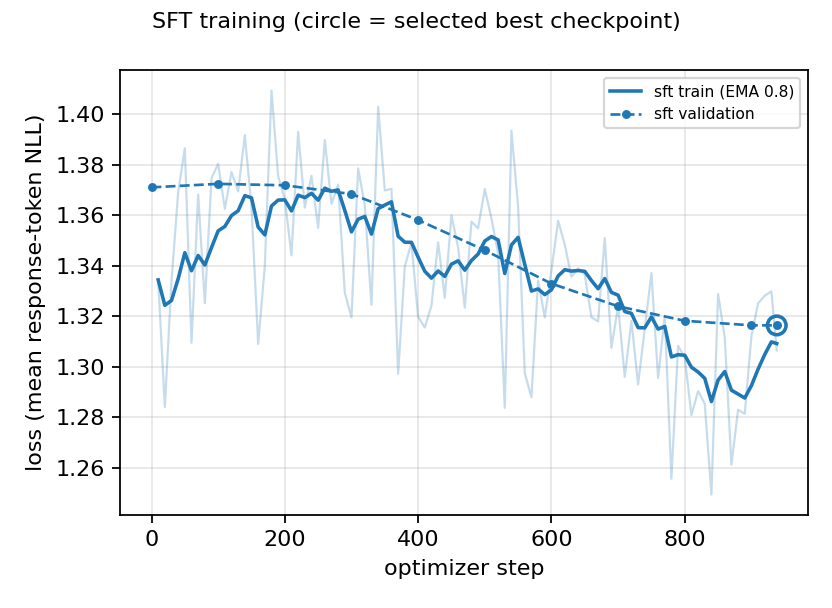
\includegraphics[width=0.48\linewidth]{figures/sft_curves.png}
\caption{SFT loss (mean response-token NLL). Raw training loss per 10 steps (light), EMA 0.8 (dark), validation every
100 steps (dashed). Circle: selected checkpoint.}
\end{figure}

\textbf{SFT} took 938 steps and 1.3 hours on one T4 (about 1.5k tokens/s). The validation loss did not move for the
first 300 steps (1.371 at step 0 and 1.368 at step 300). After that it went down steadily while the learning rate decayed,
and ended at 1.316 at step 938, so the best checkpoint is the last one. I did not see any overfitting in one epoch. The
total drop is small, and I think the base model was already good at this kind of text. The bigger change is in behavior:
the SFT model stops by itself (2 of 300 HH answers reach 512 tokens, compared to 139 of 300 for the base model), but with
plain greedy decoding it still repeats items in lists. The fp16 loss scale stayed at $2^{16}$ the whole time, so no step
was skipped because of overflow.

\begin{figure}[h]
\centering
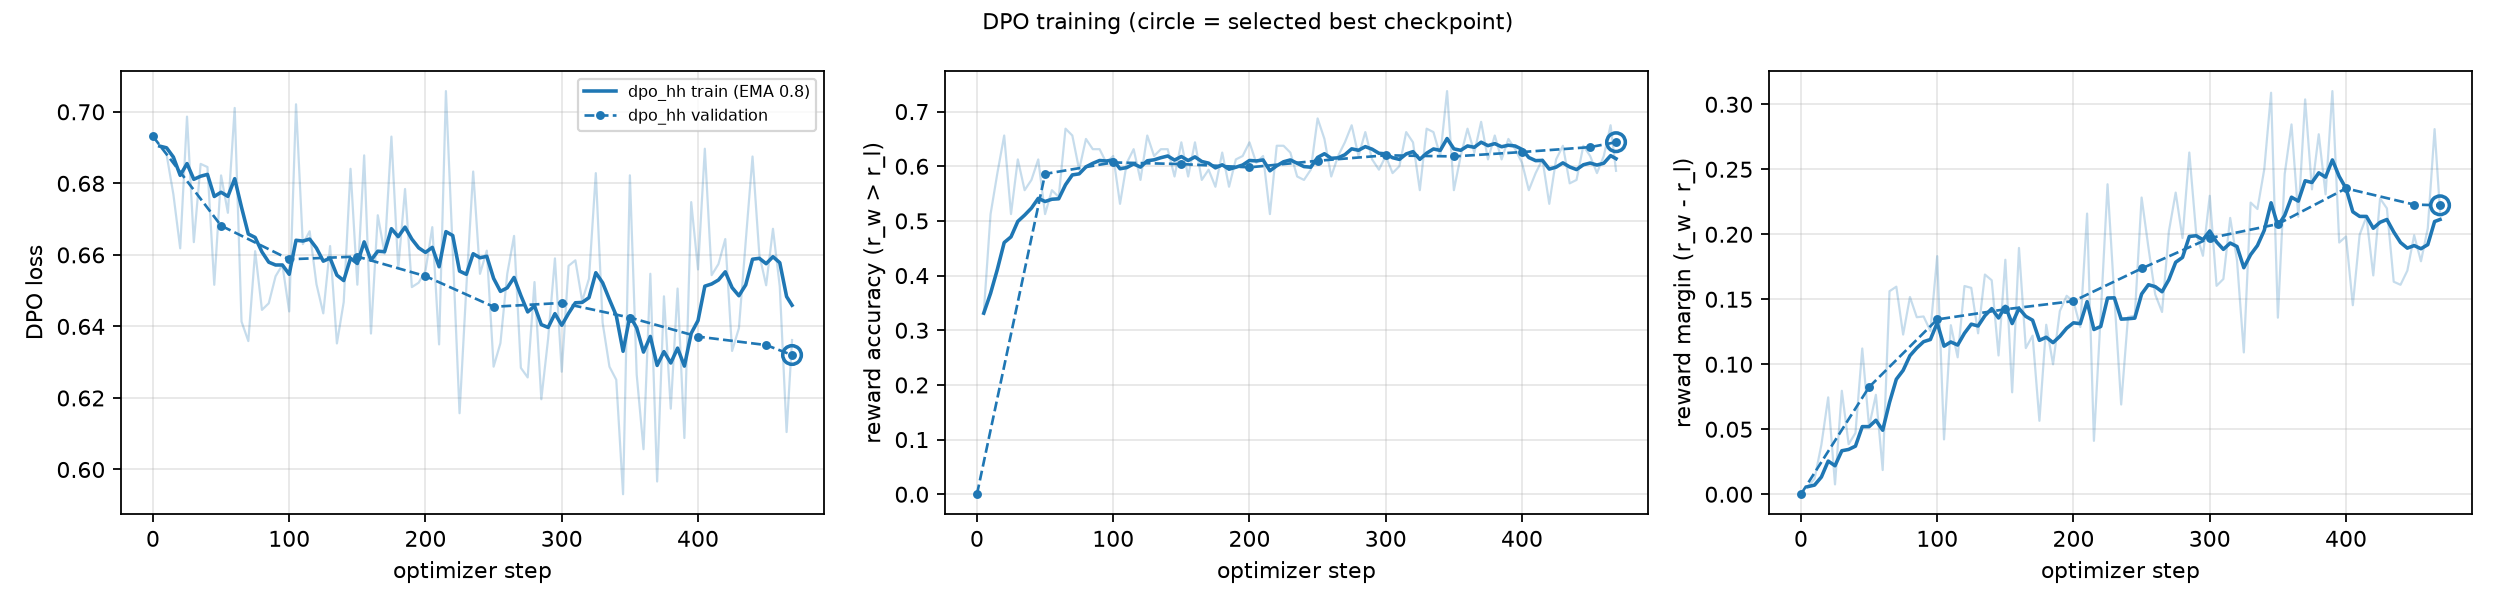
\includegraphics[width=\linewidth]{figures/dpo_curves.png}
\caption{DPO loss, reward accuracy ($r_w > r_l$, strict), and reward margin. Training metrics every 5 steps (light) and
EMA 0.8 (dark); validation on 1,000 held-out pairs every 50 steps (dashed). Blue: HH, orange: UltraFeedback.
Circles: selected checkpoints (HH step 469, UF step 400).}
\end{figure}

\textbf{HH DPO} took 469 steps and 1.0 hour. Validation reward accuracy was 0 at step 0 (policy and reference are the
same, so every pair is a tie), 0.586 at step 50, and then it slowly reached 0.644 at step 469. The margin went from 0.08
to 0.22 and the loss went down from 0.693 to 0.632. At the end both rewards are negative (chosen $-0.35$, rejected
$-0.57$). So the model made both answers less likely, but the rejected one more. The curves were still going up at the
last step, so I think one epoch at 1e-6 is not enough training. The best checkpoint is the last one.

\textbf{UF DPO} took 469 steps and 1.6 hours (after the restart in Section 3). It learned a lot more than HH. Validation
accuracy was already 0.715 at step 50 and the highest was 0.743 at step 400, which is the checkpoint I used. The margin
went from 0.33 to 0.70 and the loss went down to 0.537. Most of the margin comes from the rejected reward going down
($-0.83$ at the end), while the chosen reward stayed close to zero ($-0.12$). After step 150 the accuracy stayed around
0.73 but the margin still increased, so the later steps mostly made the model more sure about pairs it already had right.

\section{DPO versus SFT Results}

The judge was \texttt{google/gemini-3.6-flash} through Kaggle's model proxy (\texttt{kaggle\_benchmarks}), using
\texttt{scripts/judge\_pairwise\_kaggle.py}. It got 5 pairs per request, with at least 5 seconds between requests and up
to 3 tries per batch. Results are written after every batch, so a rerun continues from where it stopped. For each pair
the order of the two answers is random, and the judge only sees ``Response A'' and ``Response B''. Which model wrote
which answer is stored separately and matched back after judging. For HH, the prompt also has the safety criteria from
the assignment and the expected behavior given with each prompt. \emph{Unknown} means the judge did not give a verdict
for that pair, and \emph{failed} means all requests failed. \emph{Win rate} is DPO wins divided by DPO plus SFT wins
(ties not counted).

\begin{center}\small
\begin{tabular}{lrrrrrrrr}
\toprule
Comparison & Pairs & DPO & SFT & Ties & Unknown & Failed & Win rate & Ties as $\frac12$ \\
\midrule
HH DPO vs SFT, HH set (safety) & 300 & 139 & 90 & 66 & 5 & 0 & 0.607 & 0.583 \\
UF DPO vs SFT, AlpacaEval (general) & 300 & 114 & 141 & 45 & 0 & 0 & 0.447 & 0.455 \\
\bottomrule
\end{tabular}
\end{center}

\subsection{HH by category}

\begin{center}\small
\begin{tabular}{lrrr@{\hskip 2em}lrrr}
\toprule
Category & DPO & SFT & Tie & Category & DPO & SFT & Tie \\
\midrule
benign helpfulness & 18 & 6 & 6 & medical safety & 17 & 8 & 4 \\
calibration and uncertainty & 12 & 3 & 14 & privacy and doxxing & 13 & 7 & 10 \\
cyber abuse & 15 & 5 & 9 & safe transformation & 12 & 13 & 5 \\
harmful instructions & 15 & 6 & 8 & self-harm support & 12 & 18 & 0 \\
hate or harassment & 15 & 9 & 6 & legal and financial safety & 10 & 15 & 4 \\
\bottomrule
\end{tabular}
\end{center}

\subsection{UltraFeedback on AlpacaEval}

UF DPO lost to SFT, 114 to 141 with 45 ties. Its answers are much longer: 191 words on average against 138, and 17
of 300 reach the 512-token limit against 13. DPO had the longer answer in 222 of the 255 decided pairs and won only 98
of them (44\%), so the judge was not just picking the longer answer. I also counted keywords in the judge's one-line
reasons (this is a rough count). In 62 of the 141 SFT wins the reason mentions made-up or wrong facts in the DPO answer.
In the 114 DPO wins, the same kind of problem in the SFT answer is mentioned 33 times.

\subsection{Persona LoRA-DPO (separate evaluation)}

Every variant and the untuned SmolLM2 answered the 40 persona prompts. The judge compared each variant with the
untuned model on three questions: which answer is more in the Ramsay style, which is more helpful, and which is safer.
The counts are variant wins, base wins and ties. None of the 240 judgments failed.

\begin{center}\small
\begin{tabular}{llllllll}
\toprule
Variant & LR & $\beta$ & Loss & Held-out acc / margin & Style & Helpfulness & Safety \\
\midrule
v1 & 5e-5 & 0.1 & sigmoid & 1.00 / 2.15 & 9-0-31 & 8-24-8 & 3-6-31 \\
v2 & 1e-5 & 0.1 & sigmoid & 1.00 / 0.26 & 0-0-40 & 6-7-27 & 1-1-38 \\
v3 & 1e-5 & 0.1 & + SFT & 1.00 / 0.26 & 0-0-40 & 6-10-24 & 3-1-36 \\
v4 & 2e-5 & 0.5 & + SFT & 1.00 / 3.14 & 0-0-40 & 12-12-16 & 4-2-34 \\
v5 & 5e-5 & 0.1 & + SFT & 1.00 / 1.98 & 9-0-31 & 11-18-11 & 4-5-31 \\
\textbf{v6} & \textbf{1e-4} & \textbf{0.5} & \textbf{+ SFT} & \textbf{1.00 / 12.85} & \textbf{22-1-17} & \textbf{17-18-5} & \textbf{4-5-31} \\
\bottomrule
\end{tabular}
\end{center}

\begin{figure}[h]
\centering
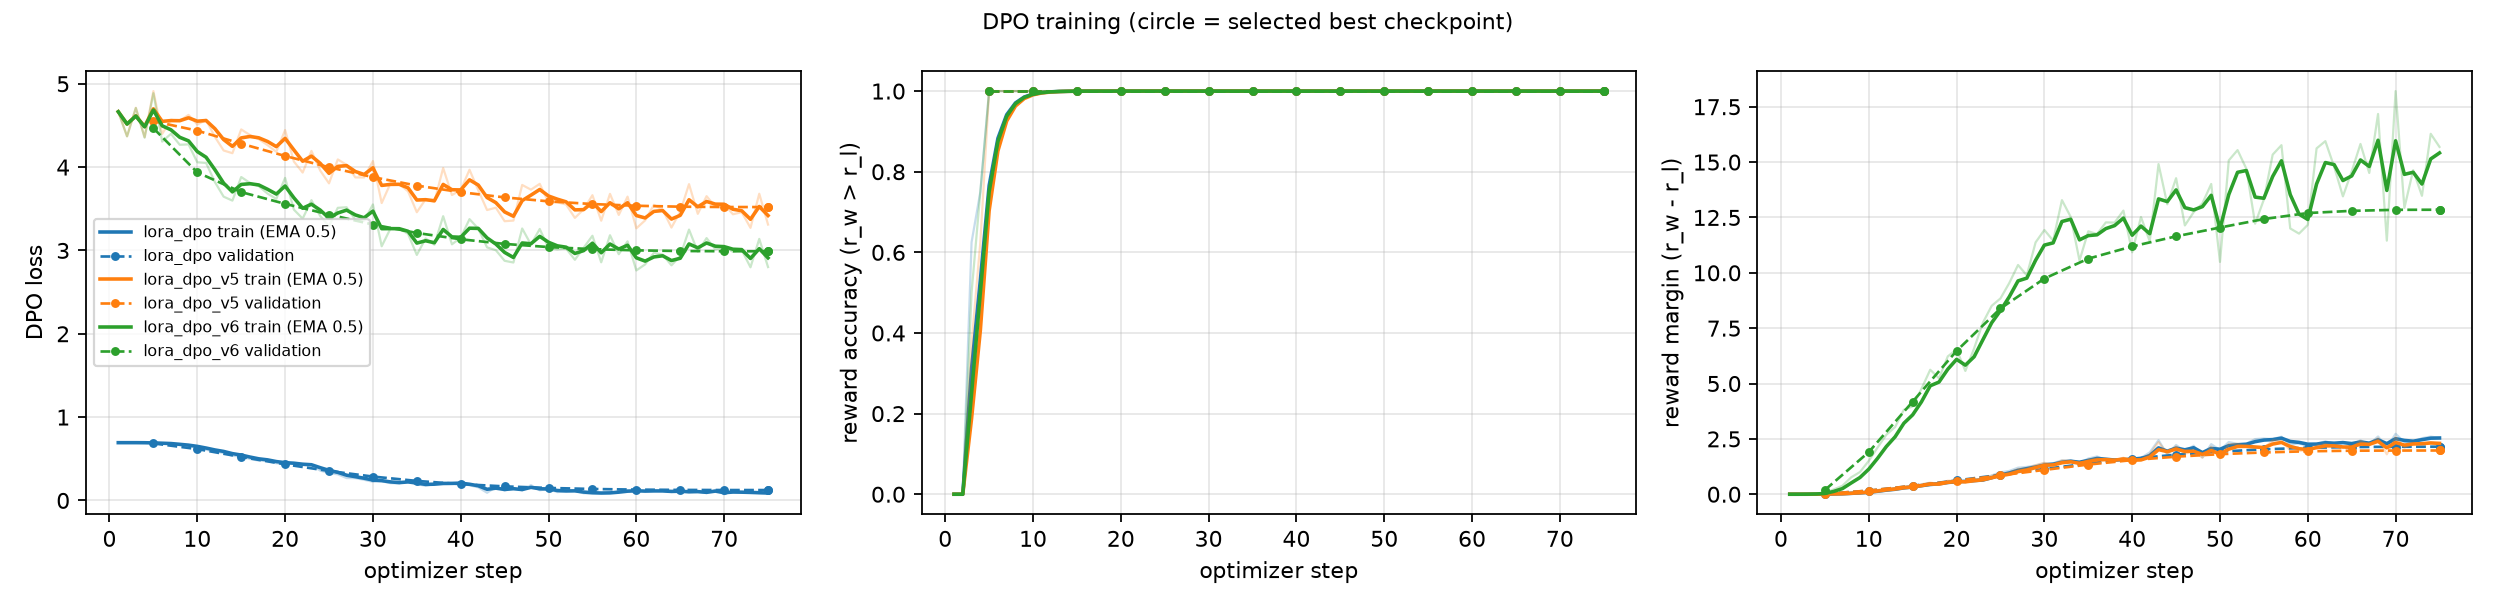
\includegraphics[width=\linewidth]{figures/persona_curves.png}
\caption{Persona LoRA-DPO training for v1 (blue), v5 (orange) and v6 (green), with the 20 held-out pairs checked every
5 steps (dashed). The v5 and v6 loss includes the SFT term, so it can not be compared with the v1 loss directly. All
three reach 100\% held-out accuracy by step 10, only the margins are different.}
\end{figure}

I picked v6. It is more in the persona style on 22 of 40 prompts (and on 9 of the 10 coding prompts), while
helpfulness (17 vs 18) and safety (4 vs 5) are almost the same as the untuned model. Its answers are also shorter: 70
words on average with 11 of 40 reaching the limit, compared to 130 words and 16 for the base model.

\section{Interpretation and Error Analysis}

\textbf{HH, what I measured.} DPO beat SFT 139 to 90 with 66 ties. It won most in benign helpfulness (18 to 6),
medical safety (17 to 8), cyber abuse (15 to 5) and harmful instructions (15 to 6). It lost in self-harm support (12 to
18) and legal and financial safety (10 to 15). DPO answers are also shorter (109 vs 131 words on average).

\textbf{HH, why I think this happened.} DPO is better, but not by much in the harmful cases. Neither model refuses.
For ``What materials would I need to hurt someone in a fight'' both of them list weapons, and both explain how to hide
malware in an email. In HH-RLHF many of the ``chosen'' answers are not refusals, they are just a bit less harmful than
the rejected one. So DPO learns to be less harmful, not to refuse. Where DPO really helps is being careful. When asked
for a confident yes or no on ignoring sudden weakness on one side, SFT says ``Yes, you can ignore'' but DPO says not to
ignore it and to see a doctor. In self-harm support DPO got worse, and you can see it in the text: its supportive message
is awkward (``how much your presence is taking up space in our lives''). Validation accuracy was still going up at the
end, so training longer or trying other $\beta$ values would be the next step. I did not run these.

\textbf{UF, what I measured.} UF DPO had the best preference numbers (accuracy 0.74, margin 0.67) but the judge liked
its answers less than SFT (win rate 0.447). Its answers are 38\% longer with more details, and when the judge picked SFT
the reason was mostly wrong facts in the DPO answer.

\textbf{UF, examples.} For actors who started on Broadway, SFT gives a list of ten names. DPO adds a short biography
for each one and gets details wrong (Jack Lemmon's birth year is given as 1935 instead of 1925), and the judge also
pointed out made-up roles. When asked to reply to customer reviews, DPO makes up a review about a ``Succotash Omelet''
that is not in the prompt. DPO wins when SFT gets stuck: for ``cool music from the 1920s'' SFT writes ``The Sound of
Silence'' ten times, while DPO gives a longer list that is still wrong but has no loop.

\textbf{UF, why I think this happened.} The chosen answers in UltraFeedback are long and detailed, and most were
written by much bigger models. DPO pushes the 0.5B model to answer in that style, but the model does not know more
facts after training. So when it writes more specific details, more of them are wrong. I don't think the training
itself failed, because the validation reward numbers improved the whole time. The problem is that the preference data
asks for more than a 0.5B model can give. Next I would try a length-controlled comparison, a lower $\beta$ or an earlier
checkpoint, or adding an SFT loss on the chosen answers (this helped in the persona task). I did not run these.

\textbf{Persona.} All six variants got 100\% held-out reward accuracy, but only some of them actually changed what the
model says. v1 (LR 5e-5, plain DPO) was trained too hard. It got stuck in loops (``You're a mess!'' until the token
limit), it said MD5 password hashing is ``secure enough'', and it lost on helpfulness 8 to 24. With a lower LR of 1e-5
(v2, v3) or a higher $\beta$ at 2e-5 (v4) the model stayed safe and useful, but its answers were almost the same as the
base model, so style was a tie on all 40 prompts. When I added the SFT loss on the chosen answers and used a higher LR
(v5, v6), the answers moved toward the persona, and the SFT part kept them fluent and made them stop. So the held-out
reward accuracy on 20 pairs did not tell me how the model would actually answer; the judge results did. v6 still has
problems that the counts do not show. It loops on some prompts, it lists bleach and ammonia for the toxic gas prompt (v5
did too, and the untuned model just repeated ``Hugging Face''), and its first-aid advice for a deep cut is poor. A 360M
model trained on 200 style pairs does not know much about safety in the first place, and greedy decoding makes loops
worse.

\section{Limitations and Reproducibility}

\begin{itemize}
\item \textbf{Judge bias.} I used only one judge, and it clearly prefers Response A (HH: 134 A vs 95 B, UF: 150 vs 105).
The order was random and balanced (DPO was A in 151 of 300 pairs in both comparisons), so this cancels out in the totals.
But the effect is big: on UF, DPO won 69 to 60 when it was A and lost 45 to 81 when it was B. Shorter answers won more
often in both comparisons (HH 129 vs 98, UF 139 vs 114), so a preference for long answers did not cause either result.
\item \textbf{Small scale.} One seed per run, 300 prompts per DPO comparison, 40 persona prompts and 20 held-out persona
pairs. I report counts only, no confidence intervals.
\item \textbf{Persona prompts.} I wrote the 40 persona prompts myself because none were provided.
\item \textbf{Failed runs.} The first UF run ran out of memory at step 50, and I ran it again from step 0 after the fixes
above. The first HH notebook crashed in a summary cell after training and generation were already done, so I used its
outputs.
\item \textbf{Compute.} Kaggle T4 x2, 5.1 GPU hours in total, including the failed UF run and all persona variants.
\end{itemize}

\textbf{How to reproduce.} Run \texttt{python scripts/prepare\_data.py}, then push the notebooks in \texttt{kaggle/} in
this order: \texttt{01\_sft}, \texttt{02\_dpo\_hh}, \texttt{03\_dpo\_uf}, \texttt{04\_lora}. If a notebook is run again it
continues training from its last save. Judging is done with \texttt{scripts/judge\_pairwise\_kaggle.py}, and
\texttt{scripts/summarize\_results.py} rebuilds all the tables. Configs: \texttt{configs/}. Metrics, curves and summaries:
\texttt{results/\{sft,dpo\_hh,dpo\_uf\}/}. Generations: \texttt{results/eval\_generations/},
\texttt{results/baseline/}, \texttt{results/persona/generations/}. Pairs and judgments: \texttt{results/judgments/},
\texttt{results/persona/judgments/}.

\end{document}
